\item \textbf{Now, explore whether you can leverage additional information in the file as exogenous variables. Use appropriate tools to evaluate the suitability of using these variables and summarize your results. There is no fixed number of variables assigned – use your judgement and justify your decisions.  Using an ARIMAX framework, show the impact of including additional variables as part of your prediction. Repeat the analysis in 2 (a) and (b) using the updated models.} 


\textit{First, we visualized the raw signals.} 

\begin{figure}[H]
    \centering
    \begin{minipage}[b]{1\textwidth}
        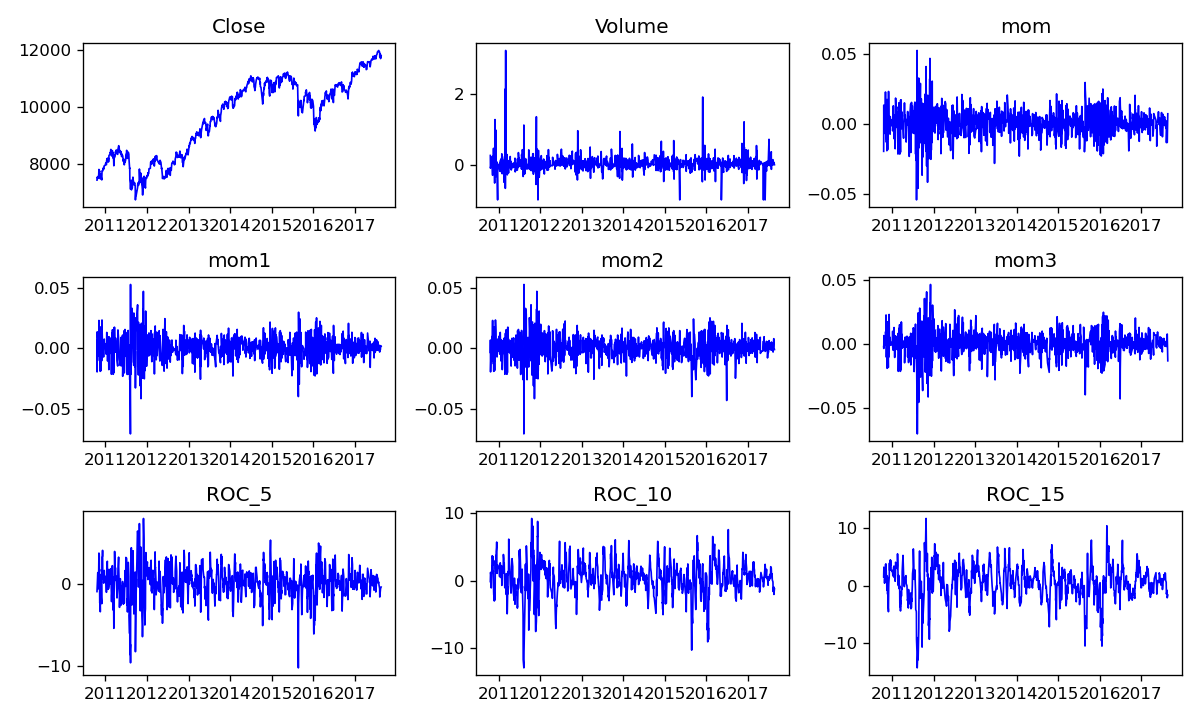
\includegraphics[width=\textwidth]{figures/Ass2/Ass2_Q3_raw_signal.png}
    \end{minipage}
    \caption{The visualization of the first nine columns.}
    \label{fig:Ass2_Q3_raw_signal}
\end{figure}


\textit{Before any transformation, we applied the Granger causality test on the first 20 variables. The null hypothesis (H0) of this test says that two variables do not Granger causes, and its alternate hypothesis (H1) indicates the second signal has a significant effect on the first signal. So, wherever P-value is less than 0.05, we can consider Grange causality. Table \ref{tab:Ass2_Q3_Granger_results1} indicates the result of this test on the first twelve columns. For this test, the maximum lag set 12.\\
Based on this test, signals mom, mom1, ROC\_X, Oil, and EMA\_X were Granger causality of the "Close price"; We stored these variables for the next steps. }

\begin{table}[H]
\centering
\caption{The result of Granger causality test.}
\label{tab:Ass2_Q3_Granger_results1}
\begin{tabular}{rlrrc}
\toprule
\# & Variable Name &  min\_p\_value &   lag &  Causality \\
\midrule
1 & Close   &       1.0000 &   1.0 &        - \\
2 & Volume  &       0.2613 &  10.0 &        - \\
3 & mom     &       0.0022 &   8.0 &        \Tik \\
4 & mom1    &       0.0285 &   7.0 &        \Tik \\
5 & mom2    &       0.2049 &   2.0 &        - \\
6 & mom3    &       0.0860 &   1.0 &        - \\
7 & ROC\_5   &       0.0024 &   1.0 &        \Tik \\
8 & ROC\_10  &       0.0036 &   1.0 &        \Tik \\
9 & ROC\_15  &       0.0037 &   1.0 &        \Tik \\
10 & ROC\_20  &       0.0010 &   9.0 &        \Tik \\
11 & EMA\_10  &       0.0021 &   1.0 &        \Tik \\
12 & EMA\_20  &       0.0014 &   1.0 &        \Tik \\
13 & EMA\_50  &       0.0008 &   9.0 &        \Tik \\
14 & EMA\_200 &       0.0035 &   9.0 &        \Tik \\
15 & DTB4WK  &       0.2096 &   1.0 &        - \\
16 & DTB3    &       0.1918 &   1.0 &        - \\
17 & DTB6    &       0.2826 &  10.0 &        - \\
18 & DGS5    &       0.5876 &   5.0 &        - \\
19 & DGS10   &       0.3805 &   5.0 &        - \\
20 & Oil     &       0.0120 &   7.0 &        \Tik \\
\bottomrule
\end{tabular}

\end{table}

\textit{As these signals had a different range, we used standardization to transform all data to scale -1 and 1. Figure \ref{fig:Ass2_Q3_standard_data} indicates the standardized variables. Also, we applied \gls{ADF} on these signals to find out that these signals were stationary or non-stationary. Table \ref{tab:Ass2_Q3_ADF_results} shows the result of this test on the dataset.}

\begin{figure}[H]
    \centering
    \begin{minipage}[b]{1\textwidth}
        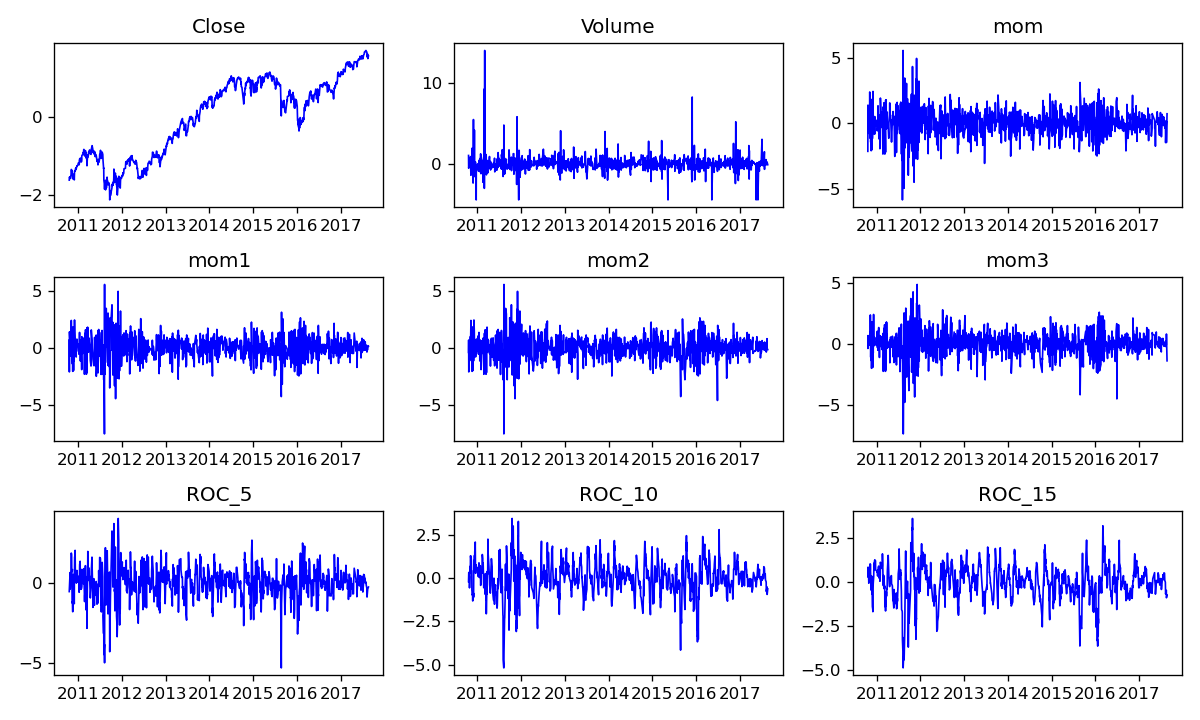
\includegraphics[width=\textwidth]{figures/Ass2/Ass2_Q4_standard_data.png}
    \end{minipage}
    \caption{The visualization of the first twelve columns. Columns were standardized.}
    \label{fig:Ass2_Q3_standard_data}
\end{figure}



\begin{table}[H]
\centering
\caption{The result of the \gls{ADF} on the dataset.}
\label{tab:Ass2_Q3_ADF_results}
{\tiny
\hspace*{-2cm}\begin{tabular}{lrrrrrrrrrrrr}
\toprule
{} &        Close &           mom &         mom1 &         ROC\_5 &        ROC\_10 &        ROC\_15 &        ROC\_20 &       EMA\_10 &       EMA\_20 &       EMA\_50 &      EMA\_200 &           Oil \\
\midrule
ADF Statistic               &    -1.085 & -12.134 &   -38.465 & -10.619 & -9.753 & -6.995 & -8.074 &    -0.967 &    -0.882 &    -0.791 &    -0.585 & -8.920 \\
p-value                     &     0.7 &  1.7e-22 &     0 &  5.5e-19 &  7.9e-17 &  7.5e-10 &  1.5e-12 &     0.7 &     0.7 &     0.8 &     0.8 &  1.0e-14 \\
\# Lags Used                  &     2 &  11 &     0 &  9 &  6 &  16 &  5 &     3 &     3 &     6 &     7 &  10 \\
\# Obs. Used &  1111 &  1102 &  1113 &  1104 &  1107 &  1097 &  1108 &  1110 &  1110 &  1107 &  1106 &  1103 \\
Critical Value (1\%)         &    -3.436 & -3.436 & -3.436 &    -3.436 & -3.436 &    -3.436 & -3.436 & -3.436 & -3.436 & -3.436 & -3.436 & -3.436 \\
Critical Value (5\%)         &    -2.864 & -2.864 & -2.864 &    -2.864 & -2.864 &    -2.864 & -2.864 & -2.864 & -2.864 & -2.864 & -2.864 & -2.864 \\
Critical Value (10\%)        &    -2.568 & -2.568 & -2.568 &    -2.568 & -2.568 &    -2.568 & -2.568 & -2.568 & -2.568 & -2.568 & -2.568 & -2.568\\
\bottomrule
\end{tabular}\hspace*{-2cm}
}
\end{table}

\textit{According to table \ref{tab:Ass2_Q3_ADF_results} all columns were stationary except the "Close price" and EMA\_X variables. Therefore, 
we used a first-order differencing to turn these time series into the stationary data. Figures \ref{fig:Ass2_Q3_1diff_Close_signal} and \ref{fig:Ass2_Q3_PACF_ACF_1diff} indicate this $1^{st}$ order differencing on "Close price" along with its \gls{ACF} and \gls{PACF} plots. These two plots also show that the data got stationary. Also, table \ref{tab:Ass2_Q3_ADF_results2} shows the ADF test on the $1^{st}$ order differencing variables.}

\begin{figure}[H]
    \centering
    \begin{minipage}[b]{1\textwidth}
        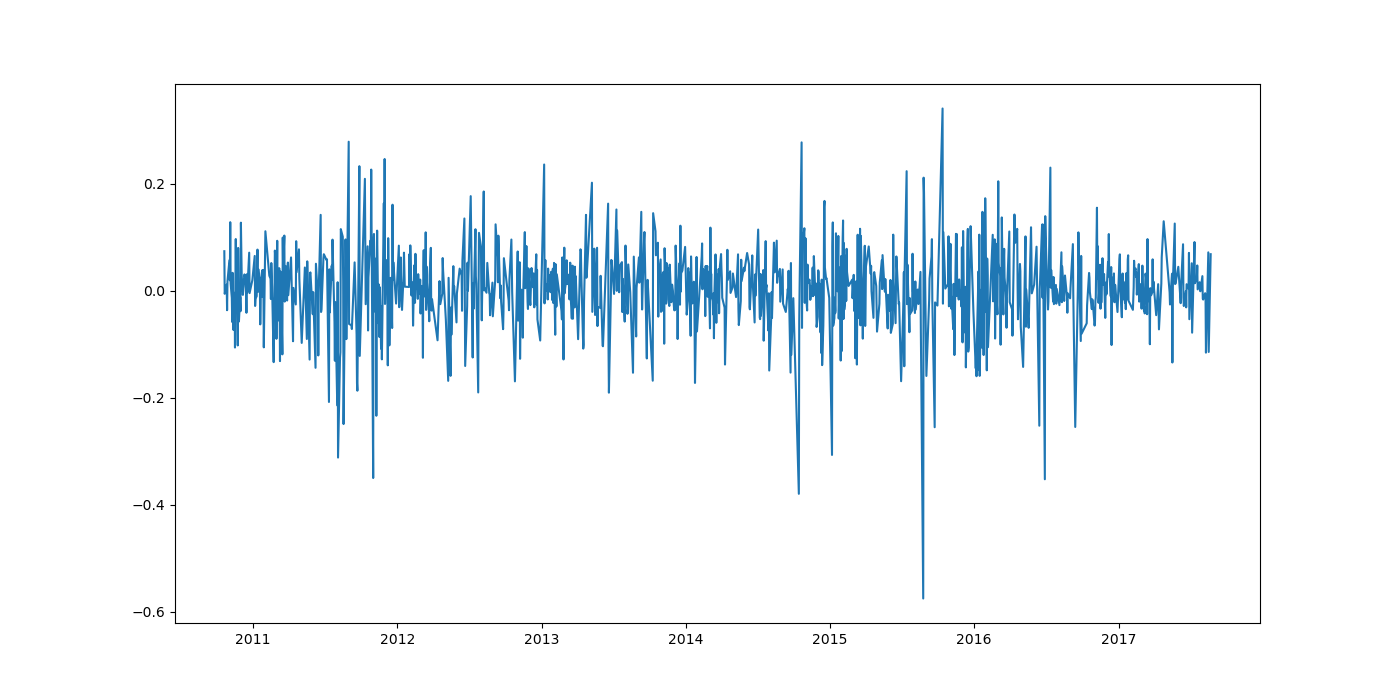
\includegraphics[width=\textwidth]{figures/Ass2/Ass2_Q3_1diff_Close_signal.png}
    \end{minipage}
    \caption{The $1^{st}$ order differencing of "Close price" data.}
    \label{fig:Ass2_Q3_1diff_Close_signal}
\end{figure}

\begin{figure}[H]
    \centering
    \begin{minipage}[b]{1\textwidth}
        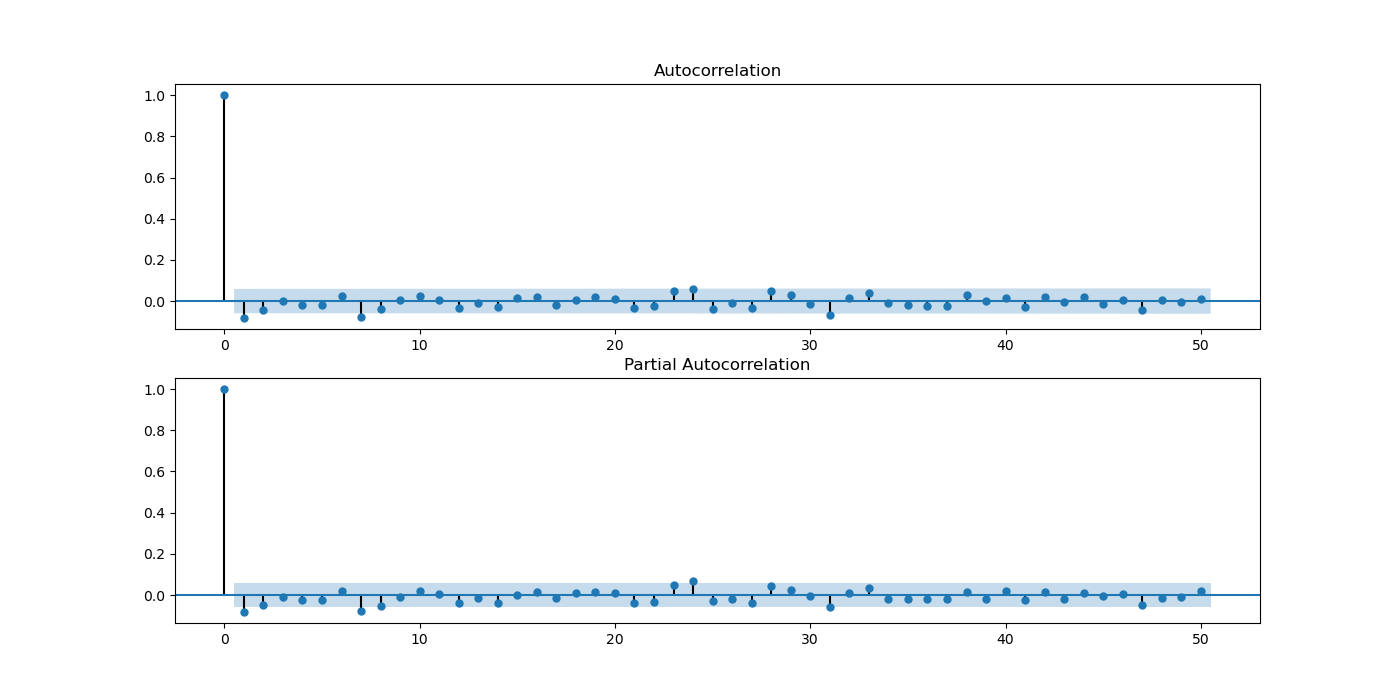
\includegraphics[width=\textwidth]{figures/Ass2/Ass2_Q3_PACF_ACF_1diff.png}
    \end{minipage}
    \caption{A plot of \gls{ACF} and \gls{PACF} on the $1^{st}$ order differencing in "Close price".}
    \label{fig:Ass2_Q3_PACF_ACF_1diff}
\end{figure}

\begin{table}[H]
\centering
\caption{The result of the \gls{ADF} on the $1^{st}$ order differencing variables.}
\label{tab:Ass2_Q3_ADF_results2}
{\tiny
\hspace*{-2cm}\begin{tabular}{lrrrrrrrrrrrr}
\toprule
{} &        Close &           mom &         mom1 &         ROC\_5 &        ROC\_10 &        ROC\_15 &        ROC\_20 &       EMA\_10 &       EMA\_20 &       EMA\_50 &      EMA\_200 &           Oil \\
\midrule
ADF Statistic               &   -25.69 & -12.13 &   -24.15 & -10.63 & -9.74 & -6.99 & -8.059 & -13.44 & -10.72 & -6.82 &    -4.72 & -8.91 \\

p-value                     &     0 &  1.7e-22 &     0 &  4.9e-19 &  8.1e-17 &  7.4e-10 &  1.6e-12 &  3.7e-25 &  3.0e-19 &  1.9e-09 &     7.6e-5 &  1.0e-14 \\
\#Lags Used                  &     1 &  11 &     1 &  9 &  6 &  16 &  5 &  2 &  2 &  5 &     6 &  10 \\
\# Observations Used &  1111 &  1101 &  1111 &  1103 &  1106 &  1096 &  1107 &  1110 &  1110 &  1.107 &  1106 &  1102 \\
Critical Value (1\%)         &    -3.436 & -3.436 & -3.436 &    -3.436 & -3.436 &    -3.436 & -3.436 & -3.436 & -3.436 & -3.436 & -3.436 & -3.436 \\
Critical Value (5\%)         &    -2.864 & -2.864 & -2.864 &    -2.864 & -2.864 &    -2.864 & -2.864 & -2.864 & -2.864 & -2.864 & -2.864 & -2.864 \\
Critical Value (10\%)        &    -2.568 & -2.568 & -2.568 &    -2.568 & -2.568 &    -2.568 & -2.568 & -2.568 & -2.568 & -2.568 & -2.568 & -2.568\\
\bottomrule
\end{tabular}\hspace*{-2cm}
}
\end{table}

\textit{After transforming and making stationary, we needed to shift exogenous variables as much as the corresponding lag in the Granger causality result.}

\textit{We fitted our model based on exogenous variables. The order of the model for this question was similar to the last question. Figure \ref{fig:Ass2_Q3_residual_plot} indicates the residual of the fitted model. As this plot illustrates, the residual signal of the model had a Gaussian distribution with zero mean. Besides, the \gls{ACF} plot shows that this signal is stationary.}



\begin{figure}[H]
    \centering
    \begin{minipage}[b]{1\textwidth}
        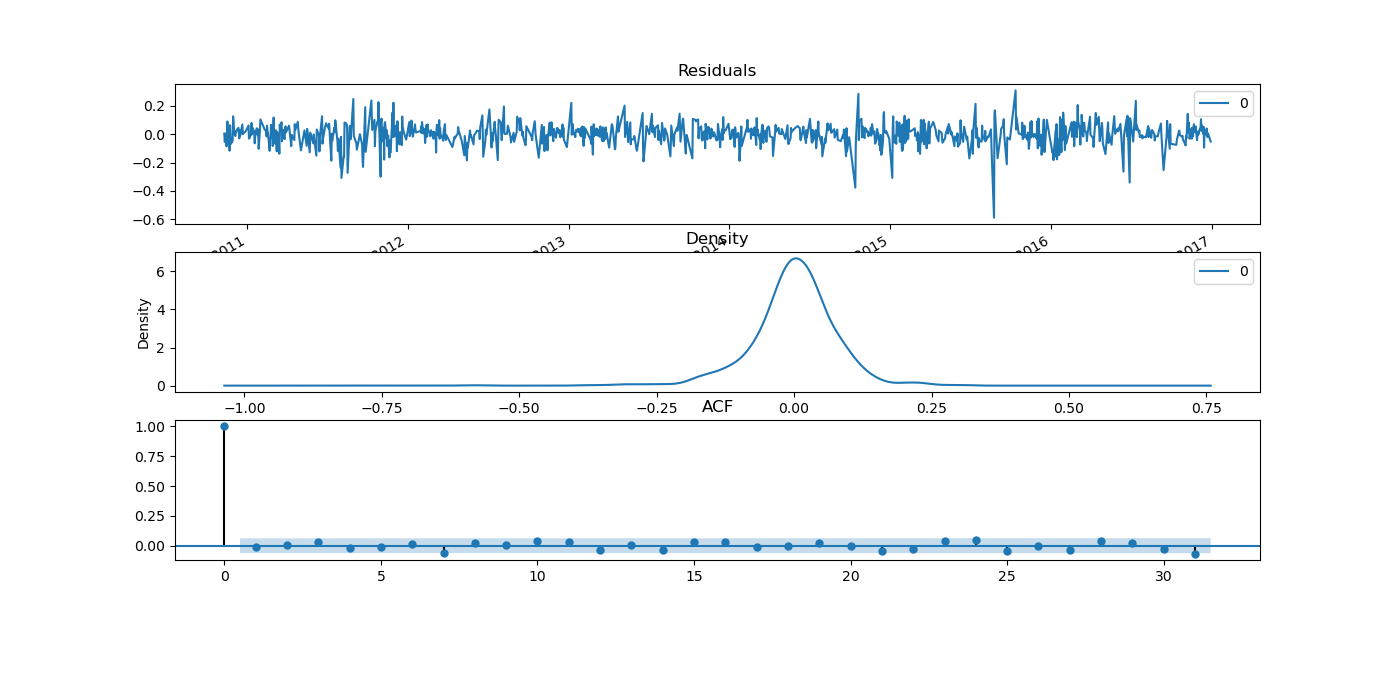
\includegraphics[width=\textwidth]{manuscript/src/figures/Ass2/Ass2_Q3_residual_plot.png}
    \end{minipage}
    \caption{The residual of the fitted model (\gls{arima}X(1, 0, 1)).}
    \label{fig:Ass2_Q3_residual_plot}
\end{figure}

\textit{To forecast, we split data into test and train set like part 2. After prediction, we needed to reverse all transformations to get the real forecast. Figure \ref{fig:Ass2_Q3_Forecast_vs_Actuals} demonstrates the output of the fitted model. As can be seen, because of using the exogenous variables, the model could predict some changes, and for others could not follow the actual data. The RMS error was 328.647.} 

\begin{figure}[H]
    \centering
    \begin{minipage}[b]{1\textwidth}
        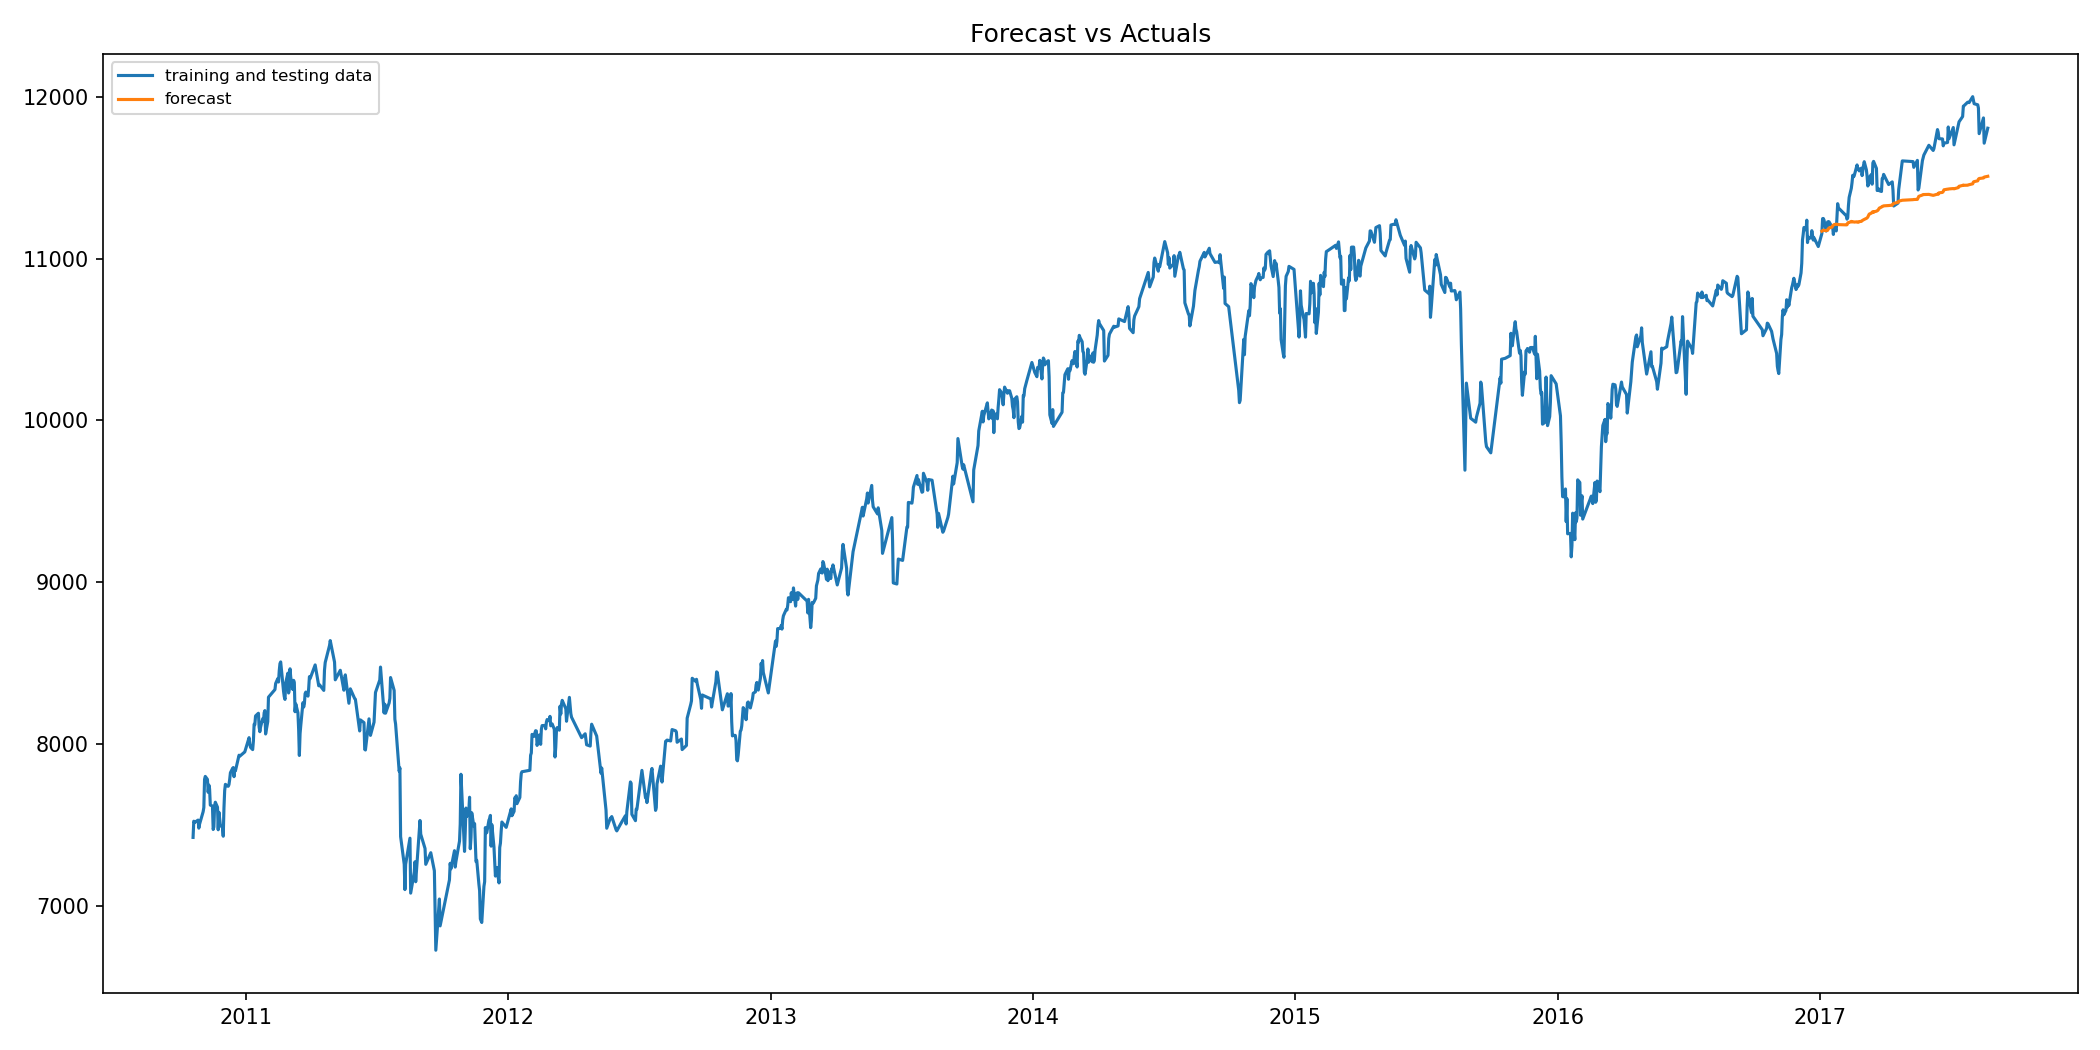
\includegraphics[width=\textwidth]{manuscript/src/figures/Ass2/Ass2_Q3_Forecast_vs_Actuals.png}
    \end{minipage}
    \caption{The prediction and actual data of \gls{arima}X(1, 0, 1) model.}
    \label{fig:Ass2_Q3_Forecast_vs_Actuals}
\end{figure}





\textit{For the rolling window approach, we used the same procedure in question 2. Figure \ref{fig:Ass2_Q3_Rolling_Forecast_vs_Actuals} demonstrates the output of the rolling window model for \gls{arima}X. As can be seen, the model could follow the test set better than previous model. The RMS error decreased from 328.647 to 256.297. It seems that the prediction of both models had a negative bias.}

\begin{figure}[H]
    \centering
    \begin{minipage}[b]{1\textwidth}
        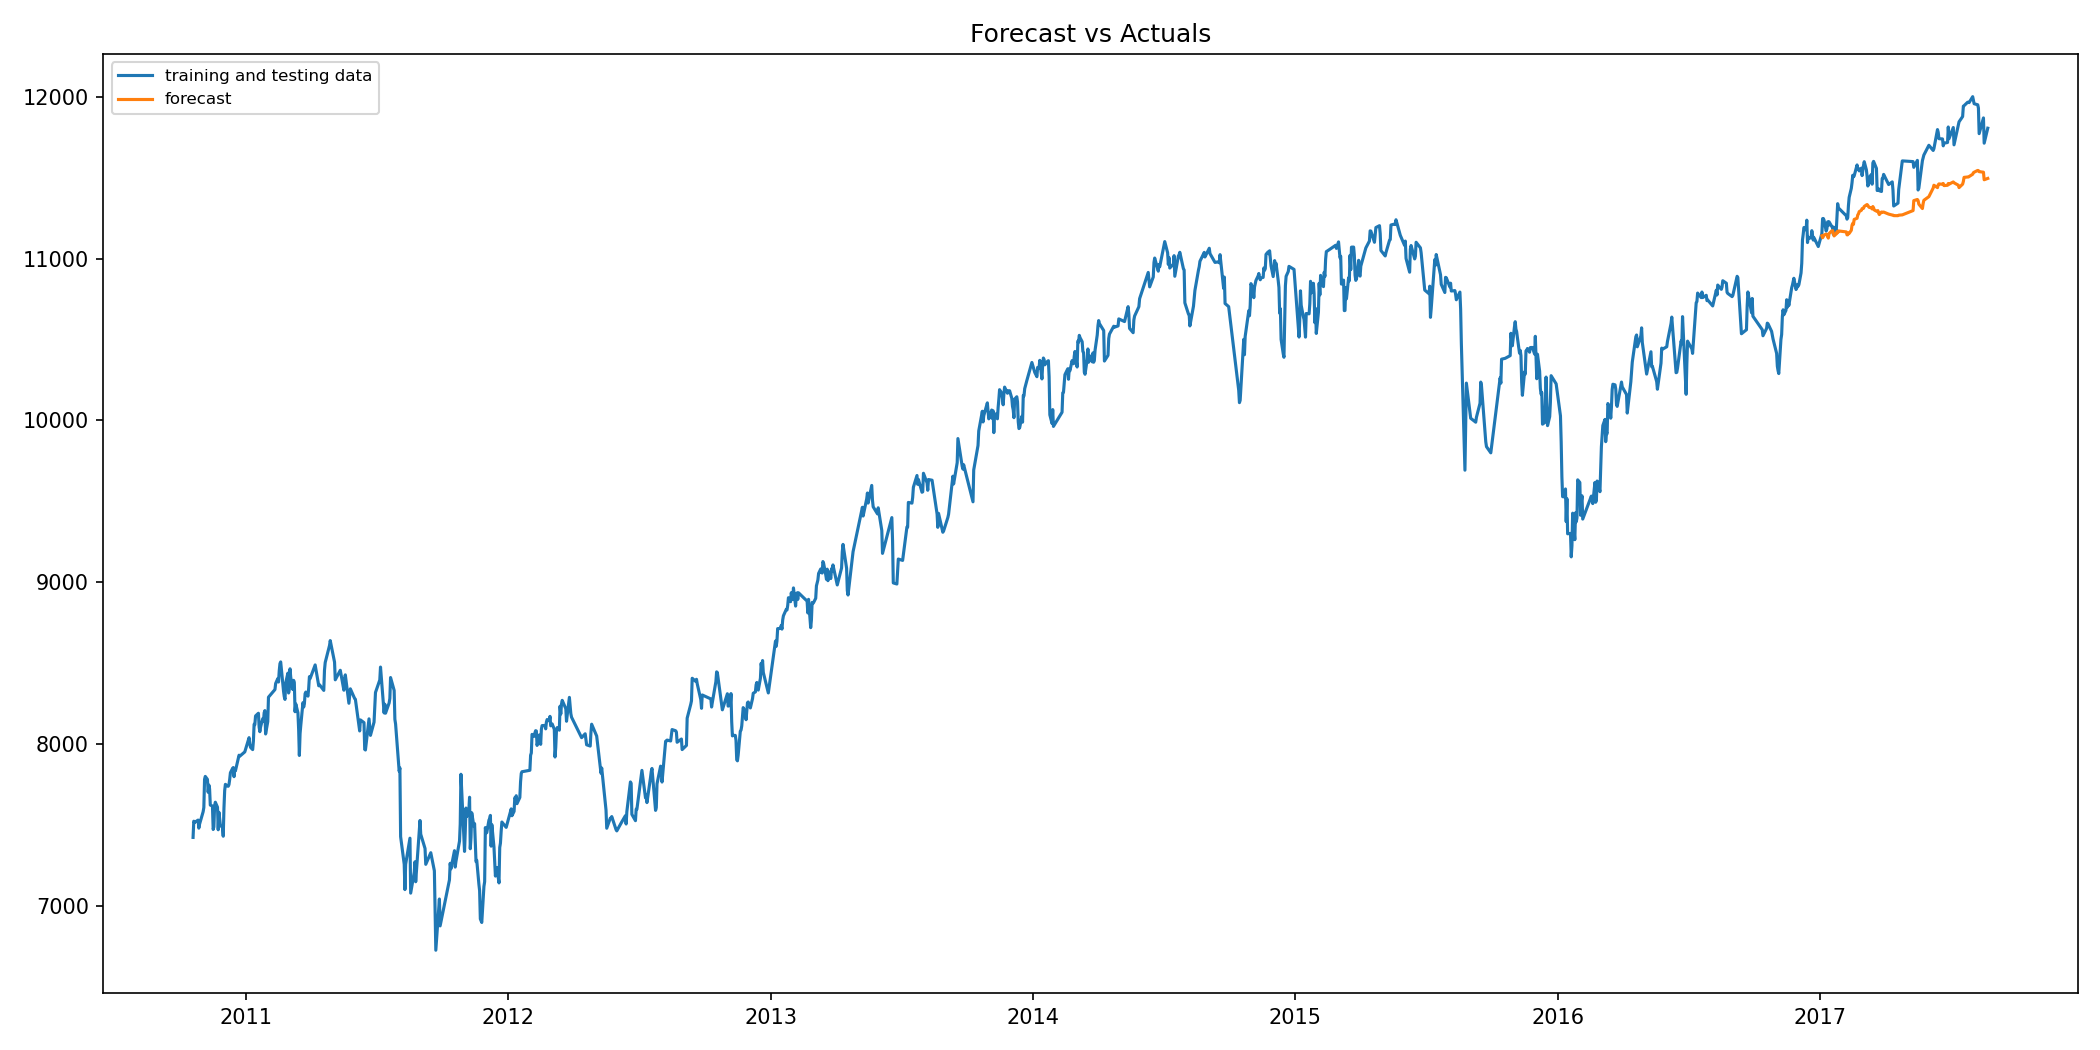
\includegraphics[width=\textwidth]{manuscript/src/figures/Ass2/Ass2_Q3_Rolling_Forecast_vs_Actuals.png}
    \end{minipage}
    \caption{The prediction and actual data of \gls{arima}X(1, 0, 1) model in rolling windows approach.}
    \label{fig:Ass2_Q3_Rolling_Forecast_vs_Actuals}
\end{figure}








